
\section{Creating a benzene dithiol (BDT) geometry}

\begin{frame}
  \frametitle{Creating a benzene dithiol (BDT) geometry}
  \tableofcontents[currentsection]
\end{frame}

\input reiterate.tex

\subsection{Electrodes}

\def\tdir{%
    \tikz \draw[->,>=latex] (0,0) -- node[right,anchor=west] {T}(0,1.5);
}

\begin{frame}
  \frametitle{Benzene dithiol (BDT)}
  \framesubtitle{Electrode}

  \begin{itemize}
    \item BDT attached to Gold electrodes
    \item We utilise 100 surface (AB-stacking)
    \item Decide $k$-point sampling in transverse direction (converge)
  \end{itemize}

  \begin{center}
    \fbox{\incg[width=.4\linewidth]{elec}}
    \hskip 2ex
    \tdir
  \end{center}

  \vskip 6ex
\end{frame}


\subsection{Molecule}

\begin{frame}
  \frametitle{Benzene dithiol (BDT)}
  \framesubtitle{BDT}

  Define the molecule

  \vskip 6ex

  \begin{columns}
    \column{.3\linewidth}
    \centering
    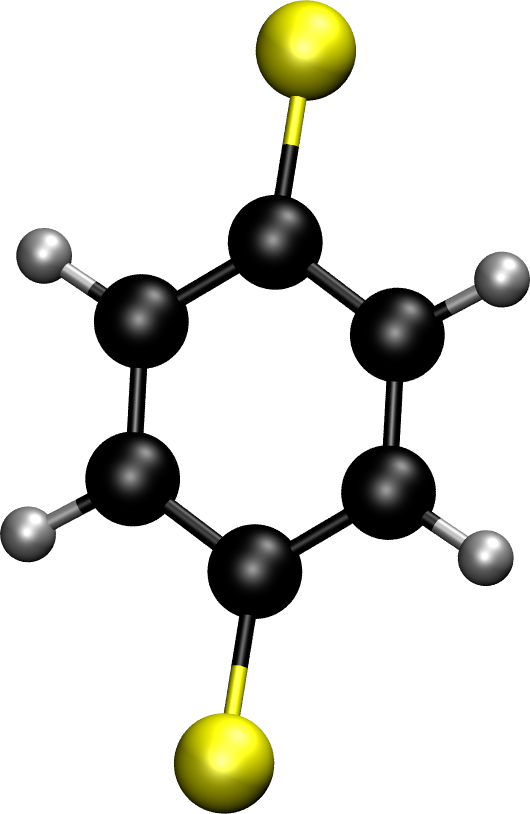
\includegraphics[height=.4\textheight]{bdt}
    \hskip 1ex
    \tdir

    \column{.7\linewidth}
    \begin{itemize}
      \item Relax structure using SIESTA
    \end{itemize}
  \end{columns}
  
\end{frame}

\subsection{Intermediate}

\begin{frame}
  \frametitle{Benzene dithiol (BDT)}
  \framesubtitle{Intermediate connect}

  Attach gold to the molecule

  \vskip 6ex

  \begin{columns}
    \column{.3\linewidth}
    \centering
    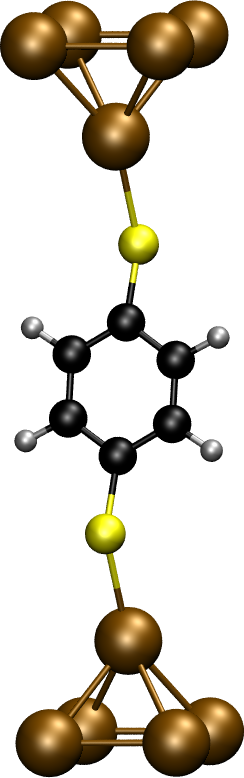
\includegraphics[height=.5\textheight]{bdt_tip}
    \hskip 1ex
    \tdir

    \column{.7\linewidth}
    \begin{itemize}
      \item Consider stacking of \emph{pyramids}
      \begin{itemize}
        \item A-BDT-A
        \item A-BDT-B
        \item B-BDT-B
      \end{itemize}
      \item Relax structure \emph{again}, constrain the \emph{pyramids}
    \end{itemize}
    
  \end{columns}

\end{frame}

\subsection{Intermediate electrode layers}

\begin{frame}
  \frametitle{Benzene dithiol (BDT)}
  \framesubtitle{Intermediate electrode layers}

  Attach a couple of electrode layers
  
  \vskip 6ex

  \begin{columns}
    \column{.3\linewidth}
    \centering
    \incg[height=.45\textheight]{bdt_tip_layer}
    \hskip 1ex
    \tdir

    \column{.7\linewidth}
    \begin{itemize}
      \item \emph{Follow} the stacking!
      \item Relax structure \emph{again}, constrain the \emph{electrode layers}
    \end{itemize}
  \end{columns}
  
\end{frame}

\subsection{Finalising simulation}

\begin{frame}
  \frametitle{Benzene dithiol (BDT)}
  \framesubtitle{Attach electrode and more intermediate layers}
  
  Attach the electrodes on both sides (converge number of intermediate layers), use
  Bloch's theorem(!)

  \vskip 3ex

  \begin{columns}
    \column{.3\linewidth}
    \centering
    \incg[height=.6\textheight]{full}
    \hskip 1ex
    \tdir

    \column{.7\linewidth}
    \begin{itemize}
      \item \emph{Follow} the stacking!
      \item Relax structure \emph{again}, constrain the \emph{electrode layers}
      \item Determining the extra number of layers:
      \begin{itemize}
        \item Consider the molecule as a ``defect''
        \item The defect has a screening length in the central region (the extra
        electrode layers)
        \item Ensure that the electrodes ``behave as bulk'' electrodes (away from defect)
      \end{itemize}
      \item<2-> What does a metallic electrode require:
      \begin{enumerate}
        \item<2-> %
        \only<3>{\color{red!50!black}}Bad screening $\to$ many extra electrode layers
        %
        \item<2-> %
        \only<3>{\color{green!50!black}}Good screening $\to$ few extra electrode layers
      \end{enumerate}
      \item<2-> What does a semi-conducting electrode require:
      \begin{enumerate}
        \item<2-> %
        \only<3>{\color{green!50!black}}Bad screening $\to$ many extra electrode layers
        %
        \item<2-> %
        \only<3>{\color{red!50!black}}Good screening $\to$ few extra electrode layers
      \end{enumerate}
    \end{itemize}
  \end{columns}
  \vskip 2ex
  
\end{frame}

%%% Local Variables:
%%% mode: latex
%%% TeX-master: "talk"
%%% End:
